\documentclass[a4paper,portuguese,10pt]{article}

\usepackage{setspace}
\usepackage[hang,footnotesize]{caption}
\usepackage[utf8]{inputenc}
\usepackage{graphicx}
%\usepackage{hyperref}
\usepackage[colorlinks=true]{hyperref}
\hypersetup{
  linkcolor=blue,
  citecolor=blue,
}
%\usepackage{setspace}
%\usepackage{abntcite}
\usepackage{amsfonts}
\usepackage{amsmath}
\usepackage{nonfloat}
\usepackage{semtrans}
\usepackage[margin=2cm]{geometry}
\usepackage[portuguese]{babel}
\usepackage[fixlanguage]{babelbib}
\selectbiblanguage{portuguese}
\usepackage[svgnames]{xcolor} % Specify colors by their 'svgnames'; list of all colors available: http://www.latextemplates.com/svgnames-colors
\usepackage{titlesec}
\usepackage[numbers]{natbib}
\usepackage{nomencl}
\usepackage{ifthen}
\usepackage{multicol} % use of multiple columns
\usepackage{fancyhdr}
\usepackage{draftwatermark}
\SetWatermarkText{PRELIMINAR}
\SetWatermarkScale{3}
%\SetWatermarkColor[rgb]{red!60}
\SetWatermarkLightness{.9}

\columnsep=8mm
%\columnseprule=1pt

\makenomenclature
% no build the list of symbols, use the following command:
% makeindex report_Leon_TUD_02-June.nlo -s nomencl.ist -o report_Leon_TUD_02-June.nls

\onehalfspacing

\newcommand{\p}{\parallel}
\newcommand{\m}{\mid}
\newcommand{\del}{\bigtriangleup}
\newcommand{\lb}{\linebreak}
\newcommand{\nl}{\newline}
%\renewcommand{\div}{{\,\rm div}\,}
\renewcommand{\div}{\nabla\cdot}
%\newcommand{\grad}{\,\rm {grad}\,}
\newcommand{\grad}{\nabla}
\renewcommand{\D}{\partial}
\newcommand{\RR}{\mathbb{R}}
\renewcommand{\vec}{\mathbf}
\newcommand{\esp}{\text{\hspace{2mm}}}
\newcommand{\dgs}{\textordmasculine}
\renewcommand{\max}{\operatorname{max}}
\newcommand{\Ra}{\operatorname{Ra}}
\renewcommand{\Re}{\operatorname{Re}}
\newcommand{\Gr}{\operatorname{Gr}}
\newcommand{\St}{\operatorname{St}}
\renewcommand{\Pr}{\operatorname{Pr}}
\newcommand{\CFL}{\operatorname{CFL}}
\newcommand{\tr}{\operatorname{tr}}

%\setlength{\hoffset}{-1cm}
%\setlength{\textwidth}{17cm}
%\setlength{\parskip}{1cm plus4mm minus3mm}
\setlength{\parskip}{2mm}
\setlength{\parindent}{0mm} % Default is 15pt.
\titleformat*{\section}{\normalsize\bfseries}
\titleformat*{\subsection}{\normalsize}

\renewcommand{\refname}{\normalsize{References}}
\renewcommand{\nomname}{List of Symbols}

\renewcommand{\nomgroup}[1]{%
\ifthenelse{\equal{#1}{R}}{\item[\textbf{Roman letters}]}{%
\ifthenelse{\equal{#1}{G}}{\item[Greek letters]}{}}}

\pagestyle{fancy}
\lhead{}
\rhead{\small{Equações de Navier-Stokes}}


%%%%%%%%%%%%%%%%%%%%%%%%%%%%%%%%%%%%%%%%%%%%%%%%%%%%%%%%%%%%%%%%%%%%%%%%%%%
\begin{document}
\thispagestyle{empty}

\thispagestyle{empty}

\begin{minipage}{0.5\linewidth}
\flushleft
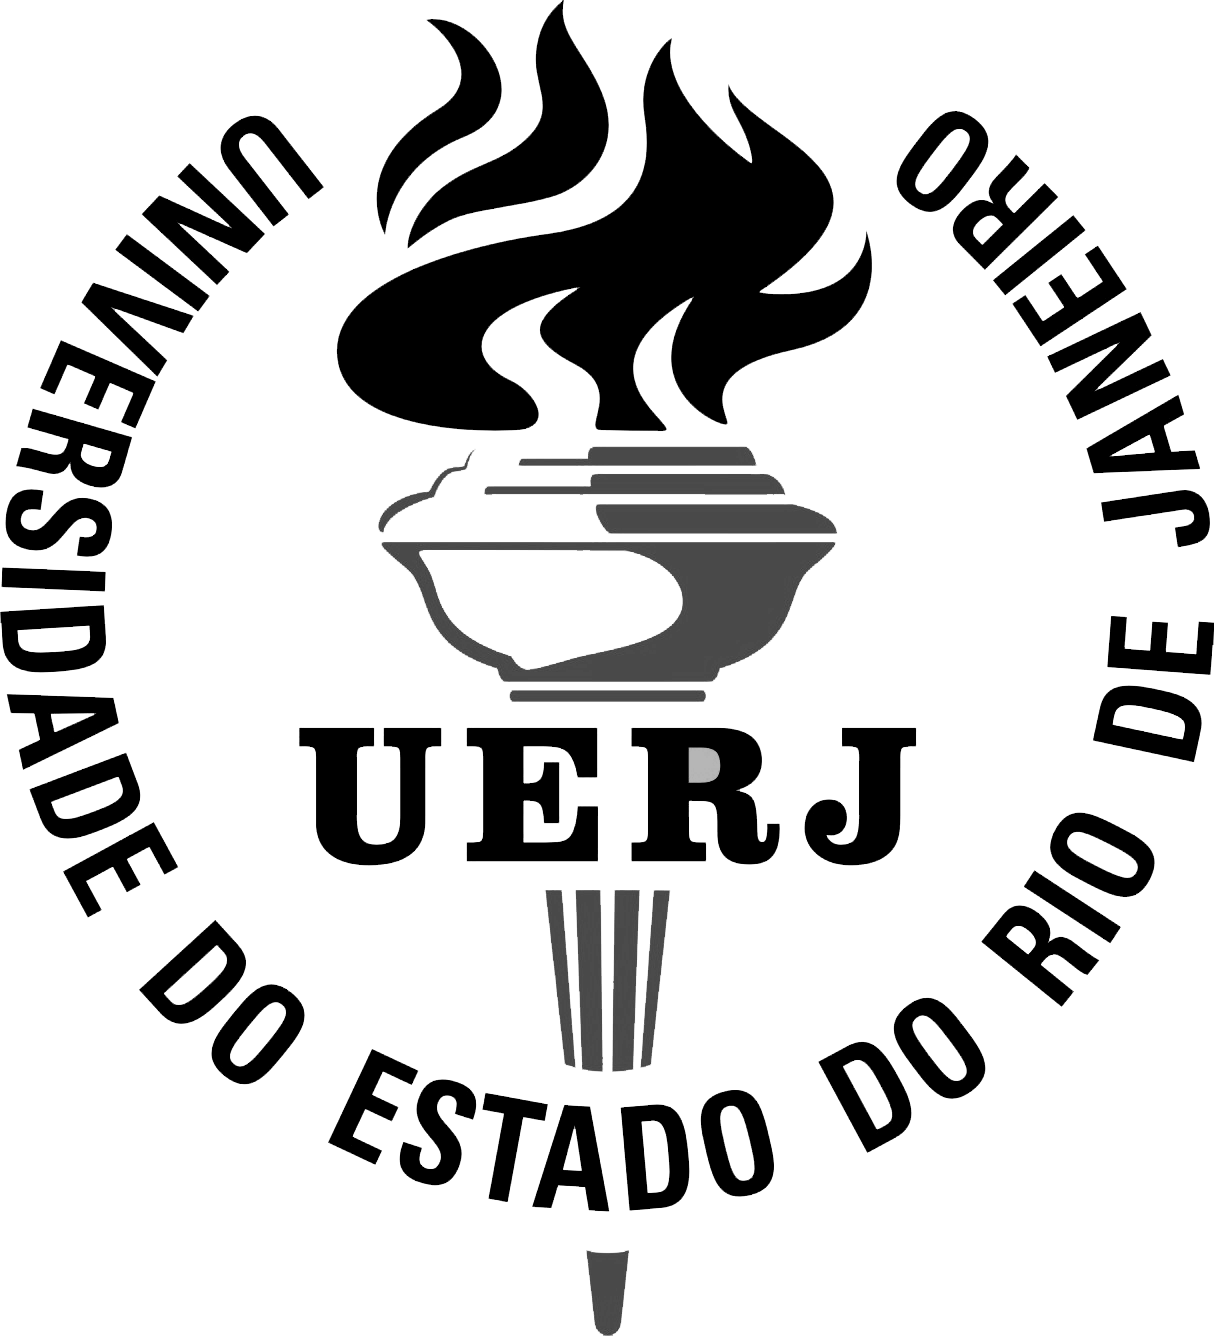
\includegraphics[height=20mm]{./figs/logo_uerj_PB.png}
\end{minipage}
\begin{minipage}{0.5\linewidth}
\flushright

\includegraphics[height=18mm]{./figs/logo_ppg-em.jpg}
\end{minipage}

\hrulefill


%\begin{center}
%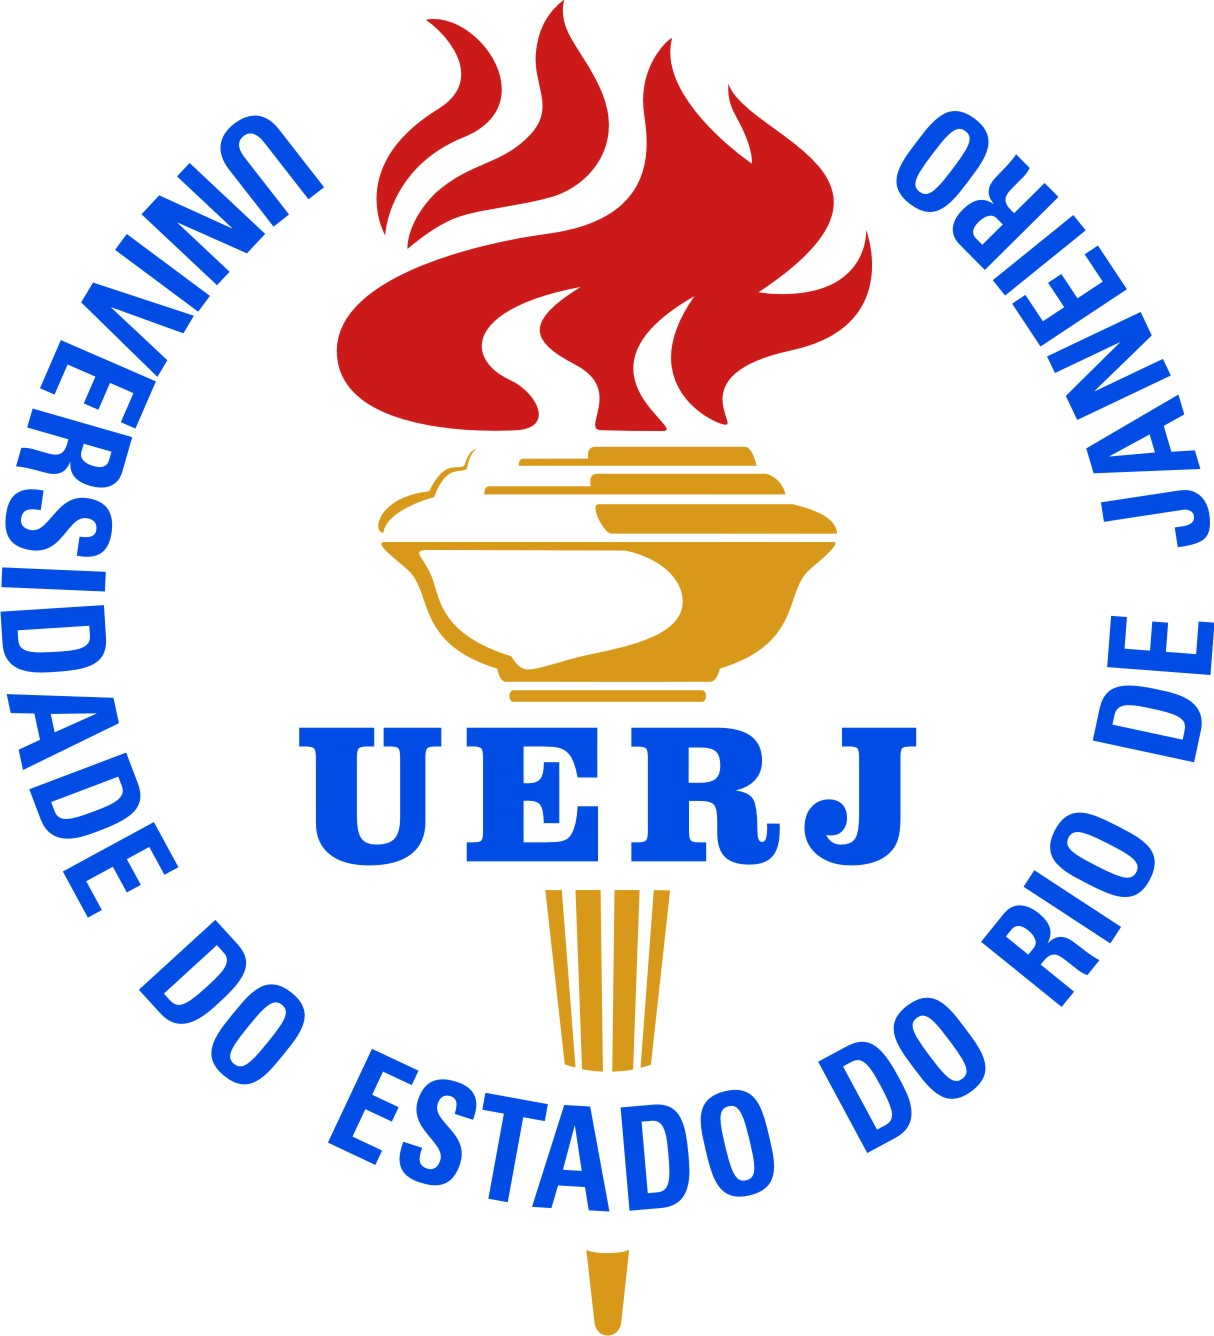
\includegraphics[scale=.3]{../../imagens/logouerj.jpg}\\
%\vspace{5mm}
%{\Large\texttt{Faculdade de Engenharia Mecânica - UERJ}}\\
%\vspace{10mm}
%\end{center}


%\vspace{5mm}
\Large \color{NavyBlue} \textbf{EQUAÇÕES DE NAVIER-STOKES}\\
\color{Black} % Title
\normalsize \texttt{Preparado por: Leon Lima}\\%[0.5cm] % Author(s)
\normalsize \texttt{\today}
\vspace{-2mm}

\setcounter{tocdepth}{1}

\hrulefill
\vspace*{-5mm}
\tableofcontents
\hrulefill

\section{Introdução}

As equações de Navier-Stokes são as mais usadas na mecânica dos fluidos. São ditas no plural -- equações -- porque são compostas por duas equações de conservação: conservação de massa de conservação de quantidade de movimento. Mas há autores que consideram apenas a conservação de quantidade de movimento como sendo a (no singular) equação de Navier-Stokes. Mesmo assim, a condição de coservação da massa deve ser sempre satisfeita. 

As equações de Navier-Stokes são:

\begin{subequations}
\begin{eqnarray}
  \frac{\D\rho}{\D t} + \div(\rho\vec{v}) &=& 0\\
  \rho\frac{\D\vec{v}}{\D t}+\rho\vec{v}\cdot\grad\vec{v} &=& -\grad P + \div[\lambda(\div\vec{v})\vec{I} + \mu\grad\vec{v}+\mu(\grad\vec{v})^T] + \vec{f}
\end{eqnarray}
\end{subequations}

Vamos agora estudar como chegamos a elas.

\section{Conservação de massa}

A equação de conservação de massa também é chamada de equação da continuidade, e pode ser escrita da seguinte forma:

\begin{equation}
  \frac{d}{dt}\int_{\Omega}\rho dV = -\int_{\D\Omega}\rho(\vec{v}\cdot\vec{n})dS
  \label{cont_int}
\end{equation}

onde $\Omega$ representa uma região no espaço e $\D\Omega$ é o contorno dessa região, $\rho$ representa densidade (massa por unidade de volume), $\vec{v}$ é o campo de velocidade e $\vec{n}$ é um vetor unitário adimensional exterior. O que essa equação diz é que a taxa temporal de variação da massa total no volume $\Omega$ é igual à quantidade de massa que entra/sai desse volume (através de seu contorno $\D\Omega$). Essa equação é dita forma integral da equação de continuidade.

Vamos agora escrever essa equação na forma local (ou diferencial). Para isso, vamos lembrar do Teorema de Green. Ele vai ser bem útil porque nos permitirá escrever as integrais de superfície, como a do lado direito da equação \ref{cont_int}, em integrais de volume. O Teorema de Green estabelece que a integral de superfície de um campo vetorial ou tensorial genérico $\vec{G}$, numa superfície fechada, é igual à integral de volume do divergente de $\vec{G}$. Ou seja:

\begin{equation}
  \int_{\D\Omega}(\vec{G}\cdot\vec{n})dS = \int_{\Omega}(\nabla\cdot\vec{G})dV
  \label{teo_green}
\end{equation}

Note que foi utilizada a notação $\nabla\cdot$ para representar o operador divergente. Se a região $\Omega$ for fixa no espaço, então ela não varia com o tempo. Essa condição, juntamente com a aplicação do Teorema de Green, nos permite reescrever a equação \ref{cont_int} como sendo

\begin{equation}
  \int_{\Omega}\frac{\D\rho}{\D t}dV = -\int_{\Omega}\div(\rho\vec{v})dV
  \label{cont_int_dif}
\end{equation}

Se a região $\Omega$ for arbitrária, então podemos escolher uma região tão pequena quanto quisermos. Em outras palavras, podemos garantir que o balanço de massa seja satisfeito em qualquer ponto do domínio. Disso resulta que

\begin{equation}
  \frac{\D\rho}{\D t} + \div(\rho\vec{v}) = 0
  \label{eq_cont_dif}
\end{equation}

Essa é a forma local da equação da continuidade. Normalmente ela é utilizada nessa forma.

\section{Equação de Conservação de Quantidade de Movimento}

O balanço de quantidade de movimento\footnote{Em inglês, quantidade de movimento é traduzida como {\it momentum}. Às vezes faz-se confusão com o termo e inglês e a quantidade de movimento é erradamente chamada de ``momento''.} consiste na condição\footnote{Essa definição foi extraída de \citet{SLATTERY99}. É possível que você se lembre da Segunda Lei de Newton a partir dessa definição. No entanto, o próprio John Slattery toma cuidado ao associar essa definição às leis de Newton (ver seção 2.2 da edição de 1999 de \cite{SLATTERY99}).} de que a taxa temporal variação da quantidade de movimento de um corpo é igual à soma das forças atuando no corpo \cite{SLATTERY99}.

\begin{equation}
  \frac{d}{dt}(m\vec{v}) = \vec{F}
  \label{balanco_qdm_01}
\end{equation}

A taxa de variação da quantidade de movimento no corpo que ocupa a região $\Omega$ pode ser escrita como sendo a soma de uma parcela relativa à derivada temporal da quantidade de movimento total e outra parcela relativa ao fluxo de quantidade de movimento que atravessa a fronteira $\D\Omega$. Vamos inserir essas parcelas na equação \ref{balanco_qdm_01}

\begin{equation}
  \frac{d}{dt}\int_{\Omega}\rho\vec{v}dV + \int_{\D\Omega}\rho\vec{v}(\vec{v}\cdot\vec{n})dS = \vec{F}
  \label{balanco_qdm_02}
\end{equation}

As forças que podem atuar no corpo são de dois tipos: forças de superfície (ou de contato) $\vec{F}_S$ e forças de corpo $\vec{F}_C$\footnote{\citet{SLATTERY99} cita um terceiro tipo de força: forças mútuas. Por exemplo, as forças intermoleculares atuando entre uma camada fina de líquido e um sólido que repousa sobre essa camada são forças mútuas. Para a maioria das aplicações de engenharia, contudo, esse tipo de força pode desconsiderado.}. Isto é, $\vec{F} = \vec{F}_S + \vec{F}_C $. As forças de superfície são resultantes das tensões que atuam na superfície do corpo. Ou seja, dado o tensor de tensões $\vec{T}$ atuando na superfície $\D\Omega$, temos que $\vec{F}_S = \int_{\D\Omega}\vec{T}\cdot\vec{n}dS$. As forças de corpo, por sua vez, são provocadas por um campo genérico $\vec{f}$ que atua em todo o volume ocupado pelo corpo. Em muitos casos este campo é a gravidade, mas pode também ser um campo magnético, por exemplo. Temos, portanto, que as forças de corpo são dadas simplesmente por $\vec{F}_C = \int_{\Omega}\vec{f}dV$. Introduzindo estas forças na equação \ref{balanco_qdm_02}, obtemos

\begin{equation}
  \frac{d}{dt}\int_{\Omega}\rho\vec{v}dV + \int_{\D\Omega}\rho\vec{v}(\vec{v}\cdot\vec{n})dS = \int_{\D\Omega}\vec{T}\cdot\vec{n}dS + \int_{\Omega}\vec{f}dV
  \label{eq_qdm_int}
\end{equation}

Essa é a forma integral da Equação de Quantidade de Movimento. Vamos agora em busca de sua forma diferencial (ou local).

Primeiro, cabe lembrar que a região é fixa no espaço, o que nos permite comutar a integração do primeiro termo com a derivada temporal. Em segundo, observe que o integrando do segundo termo do lado esquerdo pode ser escrito de uma outra forma: $\rho\vec{v}(\vec{v}\cdot\vec{n}) = \rho(\vec{v}\otimes\vec{v})\cdot\vec{n}$, onde o símbolo $\otimes$ representa produto tensorial. Vamos então reescrever o lado esquerdo da equação \ref{eq_qdm_int}.

\begin{equation}
  \int_{\Omega}\frac{\D}{\D t}(\rho\vec{v})dV + \int_{\D\Omega}\rho(\vec{v}\otimes\vec{v})\cdot\vec{n}dS = \int_{\D\Omega}\vec{T}\cdot\vec{n}dS + \int_{\Omega}\vec{f}dV
  \label{eq_qdm_int_02}
\end{equation}

Podemos, agora, aplicar novamente o Teorema de Green, porém desta vez para os tensores $\vec{v}\otimes\vec{v}$ e $\vec{T}$. Após essa operação, obtemos,

\begin{equation}
  \int_{\Omega}\frac{\D}{\D t}(\rho\vec{v})dV + \int_{\Omega}\div(\rho\vec{v}\otimes\vec{v})dV = \int_{\Omega}\div\vec{T}dV + \int_{\Omega}\vec{f}dV
  \label{eq_qdm_int_03}
\end{equation}

Se a região $\Omega$ for arbitrária, então chegamos a

\begin{equation}
  \frac{\D}{\D t}(\rho\vec{v}) + \div(\rho\vec{v}\otimes\vec{v}) = \div\vec{T} + \vec{f}
  \label{eq_qdm_int_04}
\end{equation}

Essa equação pode ser desenvolvida um pouco mais expandindo a derivada temporal e o divergente do lado esquerdo. Vamos ver como a equação \ref{eq_qdm_int_04} fica.

\begin{equation}
  \rho\frac{\D\vec{v}}{\D t} + \vec{v}\frac{\D\rho}{\D t} + \vec{v}\div(\rho\vec{v}) + \rho\vec{v}\cdot\grad\vec{v} = \div\vec{T} + \vec{f}
  \label{eq_qdm_int_05}
\end{equation}

Mas observe que, pela equação da continuidade, $\vec{v}[\frac{\D\rho}{\D t}+\div(\rho\vec{v})] = 0$. Chegamos, então, à forma local da equação de quantidade de movimento:

\begin{equation}
  \rho\frac{\D\vec{v}}{\D t} + \rho\vec{v}\cdot\grad\vec{v} = \div\vec{T} + \vec{f}
  \label{eq_qdm_dif}
\end{equation}

\section{Tensor de tensões e fluidos Newtonianos}

As forças de contato que atuam sobre um determinado corpo são conhecidas através do tensor de tensões atuantes. Quais as características desse tensor? A figura \ref{stress_tensor} mostra uma idealização de um ponto de atuação do tensor de tensões num corpo, no caso de três dimensões espaciais. Neste caso, é possível observar que o tensor possui três componentes normais, que representam as tensões normais, e seis componentes tangenciais, que representam as tensões cisalhantes (nove componentes ao total).

\begin{center}
  \includegraphics[scale=.4]{../../imagens/Components_of_Stress_Tensor.jpg}\\
  \figcaption{Representação conceitual do tensor de tensões.}
  \label{stress_tensor}
\end{center}

No entanto, o momento desse cubo diferencial deve ser nulo. Observando a figura \ref{stress_tensor}, é possível concluir que isso implica em que o tensor de tensões seja simétrico. \Citet{SLATTERY99} demonstra que o tensor de fato é simétrico calculando o momento da equação de quantidade de movimento.

Além do carater simétrico do tensor de tensões, \Citet{SLATTERY99}\footnote{É possível notar que o livro escrito por John C. Slattery é uma referência citada ao longo de todo este texto.} menciona três princípios que devem ser satisfeitos:

\begin{enumerate}
\item Princípio do determinismo: embora talvez óbvio, significa que o que ocorrer com o corpo (no futuro) não influencia no estado atual do tensor de tensões.
\item Princípio da ação local: efeitos na vizinhança de uma região arbitrariamente pequena podem ser desprezados.
\item Princípio da independência de referencial: refenciais diferentes não podem resultar em diferentes tensões.
\end{enumerate}

\citet{SLATTERY99} então apresenta uma forma geral para o tensor de tensões que satisfaz esses três princípios simultaneamente:

\begin{equation}
  \vec{T} = \kappa_0\vec{I} + \kappa_1\vec{D} + \kappa_2\vec{D}\cdot\vec{D}
  \label{eq_tensor_geral}
\end{equation}

onde $\vec{D}$ é o tensor taxa de deformação, dado por $\vec{D} = \frac{1}{2}[\grad\vec{v} + (\grad\vec{v})^T]$ (observe que ele é simétrico). A relação expressa em \ref{eq_tensor_geral} busca abranger todos os materias. Além disso, essa relação resolve a indeterminação do sistema composto por \ref{eq_cont_dif} e \ref{eq_qdm_dif}. De fato, considerando um problema 3D, por exemplo, e supondo densidade do fluido conhecida e constante, o sistema seria constituído de quatro equações -- continuidade e três componentes de quantidade de movimento -- e nove incógnitas -- três componentes de velocidade e seis do tensor de tensões\footnote{São seis, e não nove, porque ele é simétrico.}.

\subsection{Fluido Newtoniano}

Um fluido Newtoniano é caracterizado pela relação linear entre taxa de deformação e tensões. A consequência dessa definição é que $\kappa_2=0$ em \ref{eq_tensor_geral}. Os demais coeficientes de \ref{eq_tensor_geral} são $k_0=-P+\lambda\div\vec{v}$ e $\kappa_1=2\mu$ \cite{SLATTERY99}. Portanto, o tensor de tensões para um fluido Newtoniano é dado por

\begin{equation}
  \vec{T} = (-P+\lambda\div\vec{v})\vec{I} + \mu[\grad\vec{v} + (\grad\vec{v})^T]
  \label{eq_fluido_newtoniano}
\end{equation}

onde $P$ é a pressão termodinâmica, $\mu$ é a viscosidade dinâmica e $\lambda$ é a viscosidade de núcleo.

\section{\label{sec:n-s}Equações de Navier-Stokes}

As equações de Navier-Stokes são obtidas inserindo-se o tensor de tensões para fluidos Newtonianos \ref{eq_fluido_newtoniano} na equação de quantidade de movimento \ref{eq_qdm_dif}. A equação da continuidade \ref{eq_cont_dif} deve ser sempre satisfeita, por isso acompanha a equação de quantidade de movimento. Com isso, chegamos a

\begin{subequations}
\begin{eqnarray}
  \frac{\D\rho}{\D t} + \div(\rho\vec{v}) &=& 0\\
  \rho\frac{\D\vec{v}}{\D t}+\rho\vec{v}\cdot\grad\vec{v} &=& -\grad P + \div[\lambda(\div\vec{v})\vec{I} + \mu\grad\vec{v}+\mu(\grad\vec{v})^T] + \vec{f}
\end{eqnarray}
\label{eq_ns}
\end{subequations}

utilizando o fato de que $\div(P\vec{I}) = \grad P$.

Em muitos problemas de engenharia, é possível utilizar a hipótese de escoamento incompressível\footnote{Escoamento incompressível implica em densidade constante nas equações de movimento, mas não significa necessariamente que o fluido seja incompressível. Ao contrário, se o escoamento é de um fluido incompressível, o escoamento será necessariamente incompressível.}, ou seja, densidade constante. Esta condição reduz a equação da continuidade a $\div\vec{v} = 0$. Também é bastante comum que o campo de forças de corpo atuante seja a gravidade $\vec{g}$. Inserindo a conservação de massa na equação de quantidade de movimento, obtemos as equações de Navier-Stokes para escoamentos incompressíveis.

\begin{subequations}
\begin{eqnarray}
  \div\vec{v} &=& 0\\
  \rho\frac{\D\vec{v}}{\D t}+\rho\vec{v}\cdot\grad\vec{v} &=& -\grad p + \mu\grad^2\vec{v} + \vec{g}
\end{eqnarray}
\label{eq_ns_incompress}
\end{subequations}

Note que o campo de pressão na equação \ref{eq_ns_incompress} é diferente daquele da equação \ref{eq_ns}. Realmente, a hipótese de incompressibilidade não permite que a pressão termodinâmica seja definida na equação \ref{eq_ns_incompress}. A nova pressão $p$ é conhecida como pressão média, e é definida como sendo

\begin{equation}
  p = -\frac{1}{3}\tr\vec{T}
\end{equation}

onde $\tr\vec{T}$ denota o traço do tensor de tensões.

\singlespacing
%\printnomenclature

\nocite{GAMA05}

\bibliographystyle{plainnat}
\bibliography{ref}

\end{document}
